\documentclass{article}%
\usepackage[T1]{fontenc}%
\usepackage[utf8]{inputenc}%
\usepackage{lmodern}%
\usepackage{textcomp}%
\usepackage{lastpage}%
\usepackage[head=40pt,margin=0.5in,bottom=0.6in]{geometry}%
\usepackage{graphicx}%
%
\title{\textbf{OIM y Acnur exaltaron plan de trabajo para migrantes venezolanos}}%
\author{EFE}%
\date{26/11/2018}%
%
\begin{document}%
\normalsize%
\maketitle%
\textbf{URL: }%
http://www.el{-}nacional.com/noticias/mundo/oim{-}acnur{-}exaltaron{-}plan{-}trabajo{-}para{-}migrantes{-}venezolanos\_261205\newline%
%
\textbf{Periodico: }%
EN, %
ID: %
261205, %
Seccion: %
Mundo\newline%
%
\textbf{Palabras Claves: }%
NO\_TIENE\newline%
%
\textbf{Derecho: }%
18, %
Otros Derechos: %
CONTEXTO, %
Sub Derechos: %
\newline%
%
\textbf{EP: }%
NO\newline%
\newline%
%
\textbf{\textit{El Plan de Trabajo de Quito busca facilitar la movilidad humana de los ciudadanos venezolanos en Argentina, Chile, Colombia, Costa Rica, Paraguay, Perú, Uruguay y Ecuador}}%
\newline%
\newline%
%
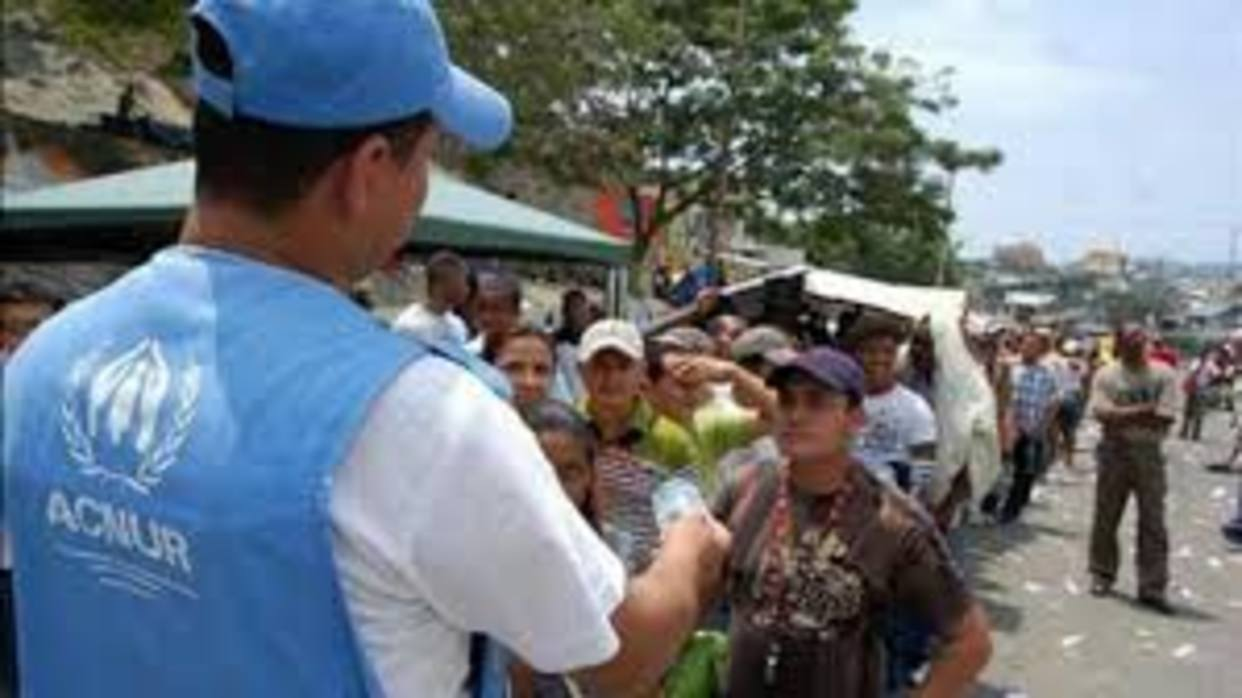
\includegraphics[width=300px]{99.jpg}%
\newline%
%
El Alto Comisionado de las Naciones Unidas para los Refugiados (Acnur) y la Organización Internacional para las Migraciones (OIM) apreciaron este lunes el plan de trabajo elaborado por ocho países latinoamericanos para atender las necesidades de los migrantes y refugiados venezolanos.%
\newline%
%
En el marco de la II Reunión Técnica Internacional, que tuvo lugar en Quito la semana pasada para tratar ese fenómeno migratorio en la región, representantes de Argentina, Chile, Colombia, Costa Rica, Paraguay, Perú, Uruguay y Ecuador suscribieron una declaración y un plan de acción para atender las necesidades de los venezolanos.%
\newline%
%
"Esta Declaración y Plan de Trabajo se inscriben en la larga tradición de solidaridad de América Latina con las personas que se ven obligadas a abandonar sus países y es un importante hito en la armonización de las políticas y prácticas de los países de la región", señaló un informe de la Acnur.%
\newline%
%
Aseguró que el Plan de Trabajo de Quito busca facilitar la movilidad humana de los ciudadanos venezolanos en los territorios de los países mencionados, quienes se comprometieron a impulsar medidas que permitan evaluar y normalizar el estatus migratorio.%
\newline%
%
También se establecen procedimientos o protocolos para garantizar el adecuado ejercicio de los derechos básicos como la salud, la educación y el trabajo para refugiados y migrantes de Venezuela.%
\newline%
%
Además, señala que los grupos de atención preferentes serán los niños y niñas, sobrevivientes de violencia sexual basada en género, personas con discapacidad y víctimas de trata.%
\newline%
%
El número de refugiados y migrantes de Venezuela en todo el mundo es de 3.000.000, incluidos 2.400.000 en América Latina y el Caribe, según el informe del Acnur.%
\newline%
%
\end{document}